\documentclass[12pt,openany,oneside,a4paper]{abntex2}
\usepackage[portuguese]{babel}
\usepackage{amsmath}
\usepackage{graphicx}
\usepackage{lipsum}
\usepackage{circuitikz}
\usepackage{icomma}
\usepackage{tikz}
\usepackage{float}

\titulo{Diagnóstico Inicial}
\autor{Matheus Amaral da Costa}
\data{Março de 2025}
\instituicao{%
  Centro Universitário FAESA
  \par
  Engenharia da Computação}
\local{Vitória, ES}

\begin{document}

\imprimircapa
\imprimirfolhaderosto*

\tableofcontents

\chapter{Análise DC}
\section{Considerações Iniciais}
Considerar que os capacitores estão "abertos".

\section{Simplificação do Circuito}
\begin{figure}[h]
  \centering
  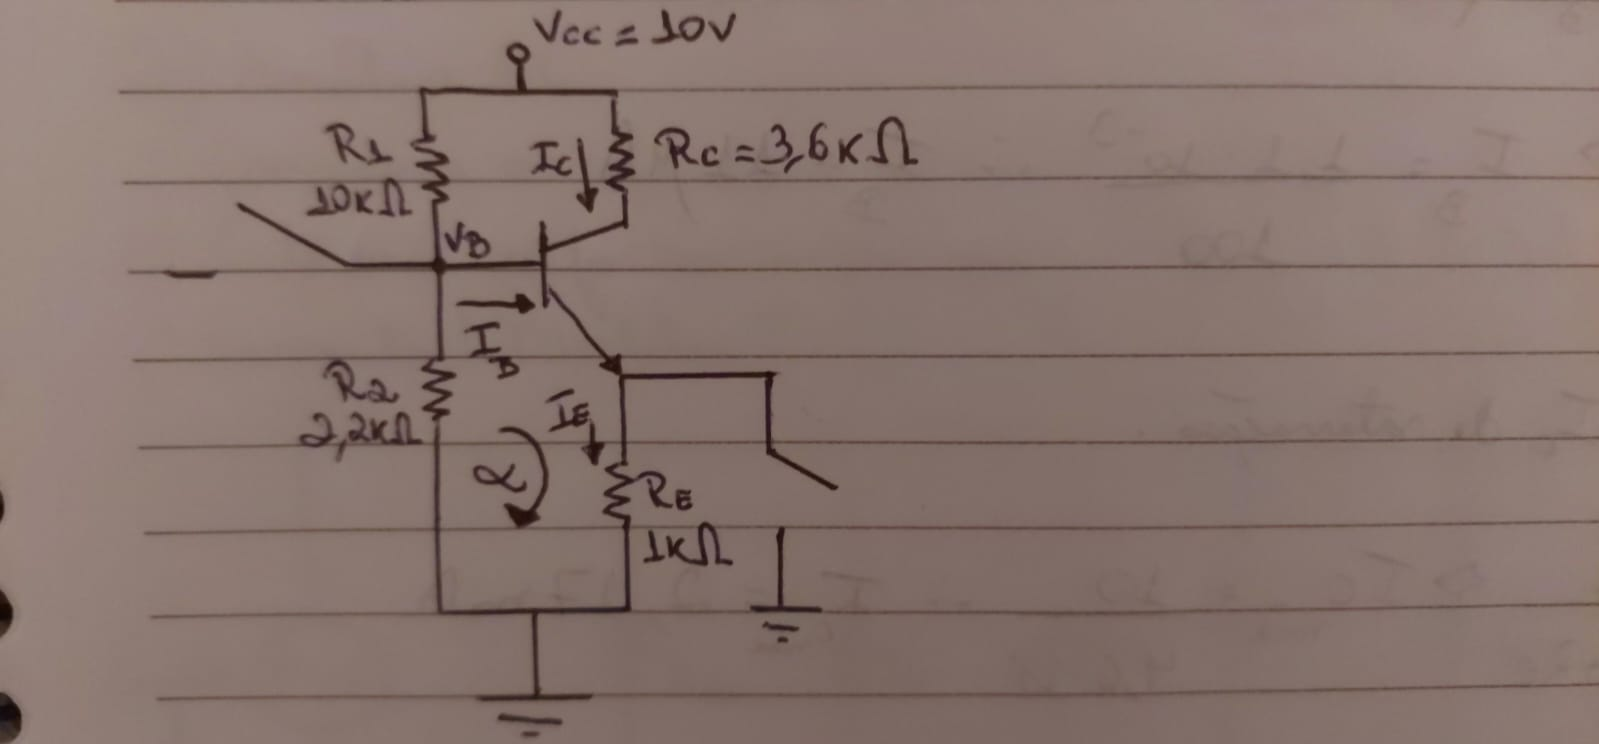
\includegraphics[width=\linewidth]{f1.jpeg}
  \caption{Circuito Simplificado}
  \label{fig:exemplo}
\end{figure}

\section{Dados do Circuito}
\begin{itemize}
    \item $V_{CC} = 10V$
    \item $R_1 = 10\,\text{k}\Omega$
    \item $R_2 = 2{,}2\,\text{k}\Omega$
    \item $R_C = 3{,}6 \, \text{k}\Omega$
    \item $R_E = 1 \, \text{k}\Omega$
    \item $R_L = 10 \, \text{k}\Omega$
\end{itemize}

\section{Determinação de $V_B$}
\[
V_B = V_{CC} \times \left(\frac{R_2}{R_1 + R_2}\right)
\]
\[
V_B = 10 \times (\frac{2{,}2 \times 10^3}{12{,}2 \times 10^3})
\]
\[
\tikz[baseline]{\node[draw=red, thick, rounded corners] {$V_B = 1{,}8\,V$};}
\]

\section{Cálculo de $I_E$}
Aplicando LKT na malha $\alpha$, tem-se:
\[
V_B - V_{BE} - R_E \cdot I_E = 0
\]
Se o diodo é de Silício, tem-se que $V_{BE} = 0{,}7V$, logo:
\[
1{,}8 - 0{,}7 - 1000 \cdot I = 0 \implies I_E = \frac{1{,}1}{1000} \implies \tikz[baseline]{\node[draw=red, thick, rounded corners] {$I_E = 1{,}1 \, \text{mA}$};}
\]

\section{Cálculo de $I_C$}
Para $\beta >= 100$, temos que $I_C \approx I_E \implies \tikz[baseline]{\node[draw=red, thick, rounded corners] {$I_C = 1{,}1 \, \text{mA}$};}$

\section{Cálculo de $I_B$}
Adotando $\beta$ = 100, temos: 
\[
I_B = \frac{I_C}{\beta} = \frac{1{,}1 \times 10^3}{100} \implies \tikz[baseline]{\node[draw=red, thick, rounded corners] {$I_B = 11 \, \text{µA}$};}
\]

\section{Cálculo do $I_C$ de Saturação}
\[
I_{Cmáx} = \frac{V_{CC}}{R_C + R_E} = \frac{10}{4{,}6 \times 10^3} \implies \tikz[baseline]{\node[draw=red, thick, rounded corners] {$I_{Cmáx} = 2{,}17 \, \text{mA}$};}
\]

\section{Cálculo do $V_{CE}$}
\[
V_{CE} = V_{CC} - R_C I_C - R_E I_E
\]
\[
V_{CE} = 10 - (R_C + R_E) \cdot 1{,}1 \times 10^{-3} \implies V_{CE} = 10 - 5{,}06 \implies \tikz[baseline]{\node[draw=red, thick, rounded corners] {$V_{CE} = 4{,}94 \, \text{V}$};}
\]

\section{Gráfico $I_{C}$ x $V_{CE}$}
\begin{figure}[H]
  \centering
  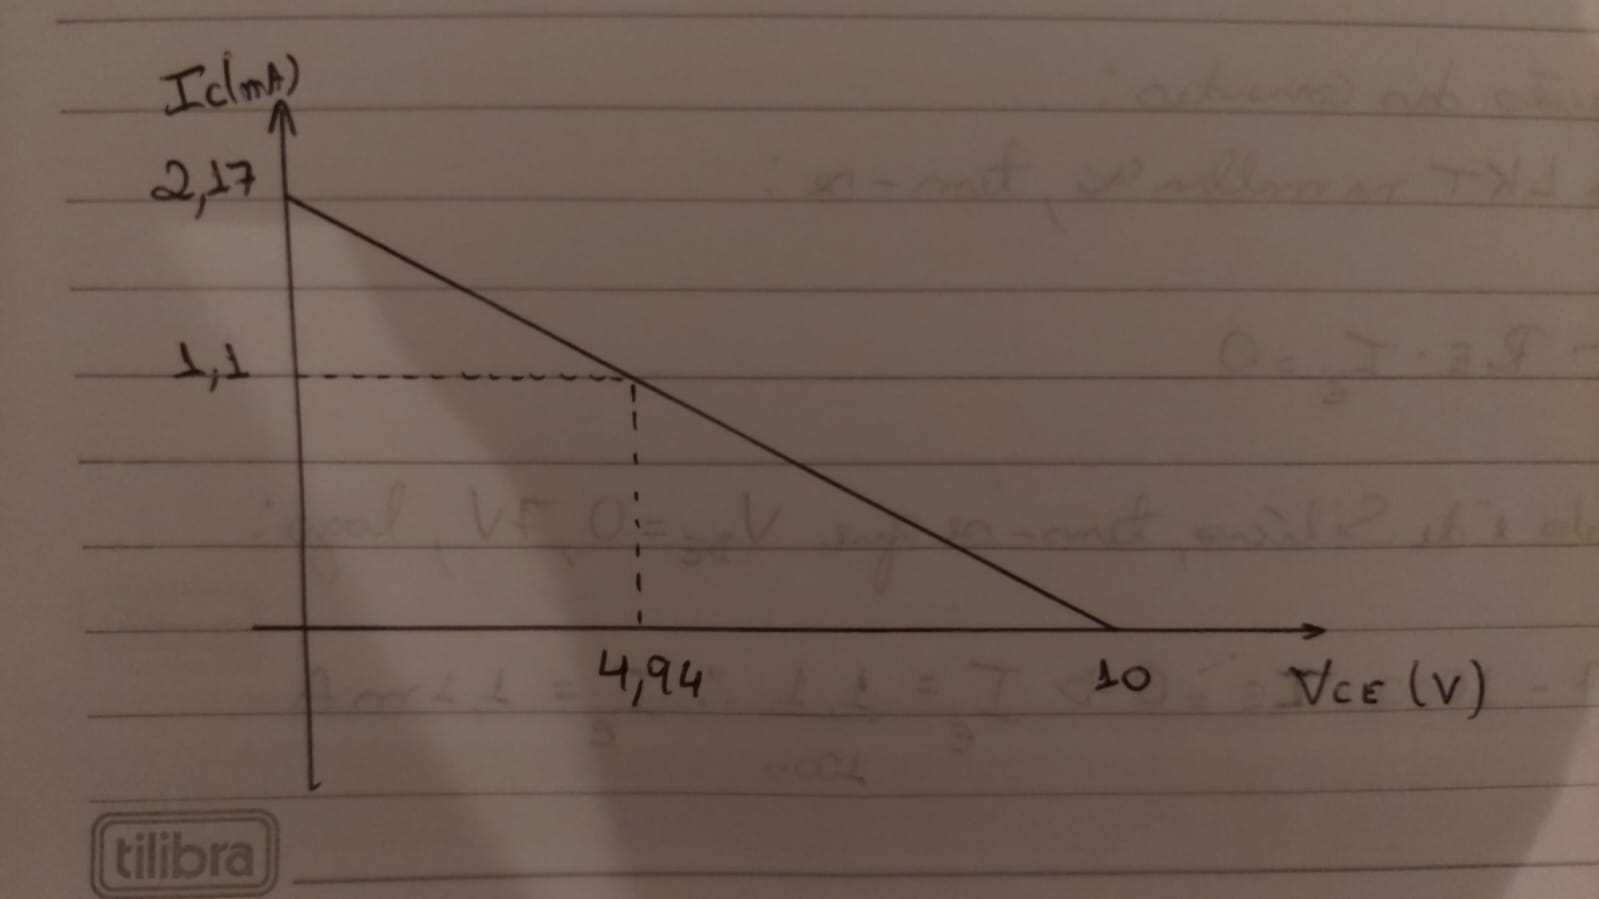
\includegraphics[width=\linewidth]{f2.jpeg}
  \caption{Gráfico $I_{C}$ x $V_{CE}$}
  \label{fig:exemplo}
\end{figure}

\section{Conclusão}
Devido ao fato de $I_{C}$ ser menor que 2{,}17 mA ($I_{C\text{máx}}$) e ser diferente de zero, a configuração está funcionando como um amplificador.

\chapter{Análise AC}
\section{Considerações Iniciais}
Considerar os capacitores em curto-circuito; \\
Aterrar as fontes contínuas.

\section{Simplificação do Circuito (Modelo Pi)}
\begin{figure}[h]
  \centering
  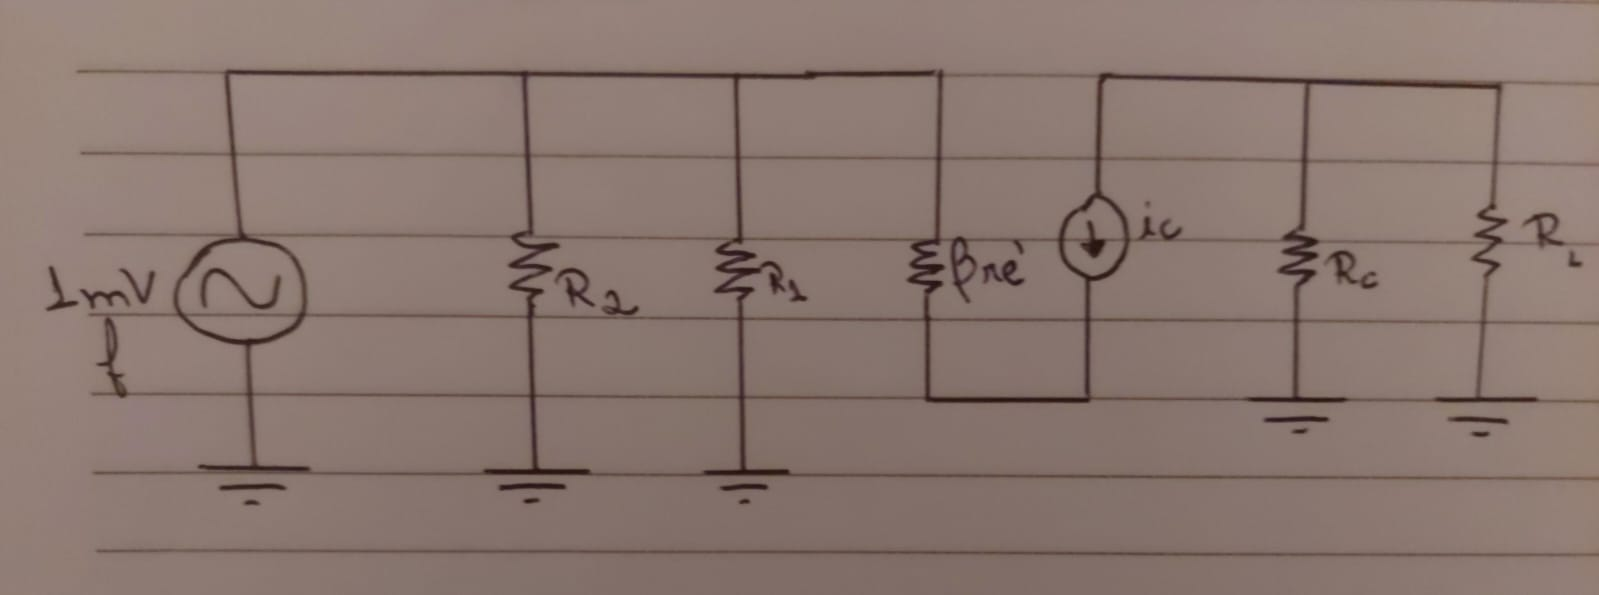
\includegraphics[width=\linewidth]{f3.jpeg}
  \caption{Circuito Simplificado (Modelo Pi)}
  \label{fig:exemplo}
\end{figure}

\section{Cálculo de $r_c$}
\[
r_c = {R_C \parallel R_L} \implies r_c = \frac{R_C \cdot R_L}{R_C + R_L}
\]
\[
r_c = \frac{10 \, \text{k}\Omega \times 3{,}6 \, \text{k}\Omega}{10 \, \text{k}\Omega + 3{,}6 \, \text{k}\Omega}
\]
\[
\tikz[baseline]{\node[draw=red, thick, rounded corners] {$r_c = 2{,}65 \, \text{k}\Omega$};}
\]

\section{Cálculo de $r_e'$}
\[
r_e^{\prime} = \frac{25 \, \text{mV}}{I_E} = \frac{25 \times 10^{-3}}{1{,}1 \times 10^{-3}} \implies \tikz[baseline]{\node[draw=red, thick, rounded corners] {$r_e^{\prime} = 22{,}72 \, \Omega$};}
\]

\section{Cálculo do Amplificador de Tensão}
\[
A_v = \frac{r_c}{r_e'} = \frac{2{,}65 \times 10^3}{22{,}72} \implies \tikz[baseline]{\node[draw=red, thick, rounded corners] {$A_v = 116{,}64$};}
\]

\section{Cálculo do ganho (em decibéis) da configuração}
\[
A_{v\text{dB}} = 20 \log_{10} A_v \implies A_{v\text{dB}} = 20 \log_{10} 116{,}64 \implies \tikz[baseline]{\node[draw=red, thick, rounded corners] {$A_{v\text{dB}} = 41{,}3 \, \text{dB}$};}
\]

\end{document}
